\documentclass[tikz, border=10pt]{standalone}
\usetikzlibrary{shapes.geometric, arrows.meta, positioning, calc}

\begin{document}

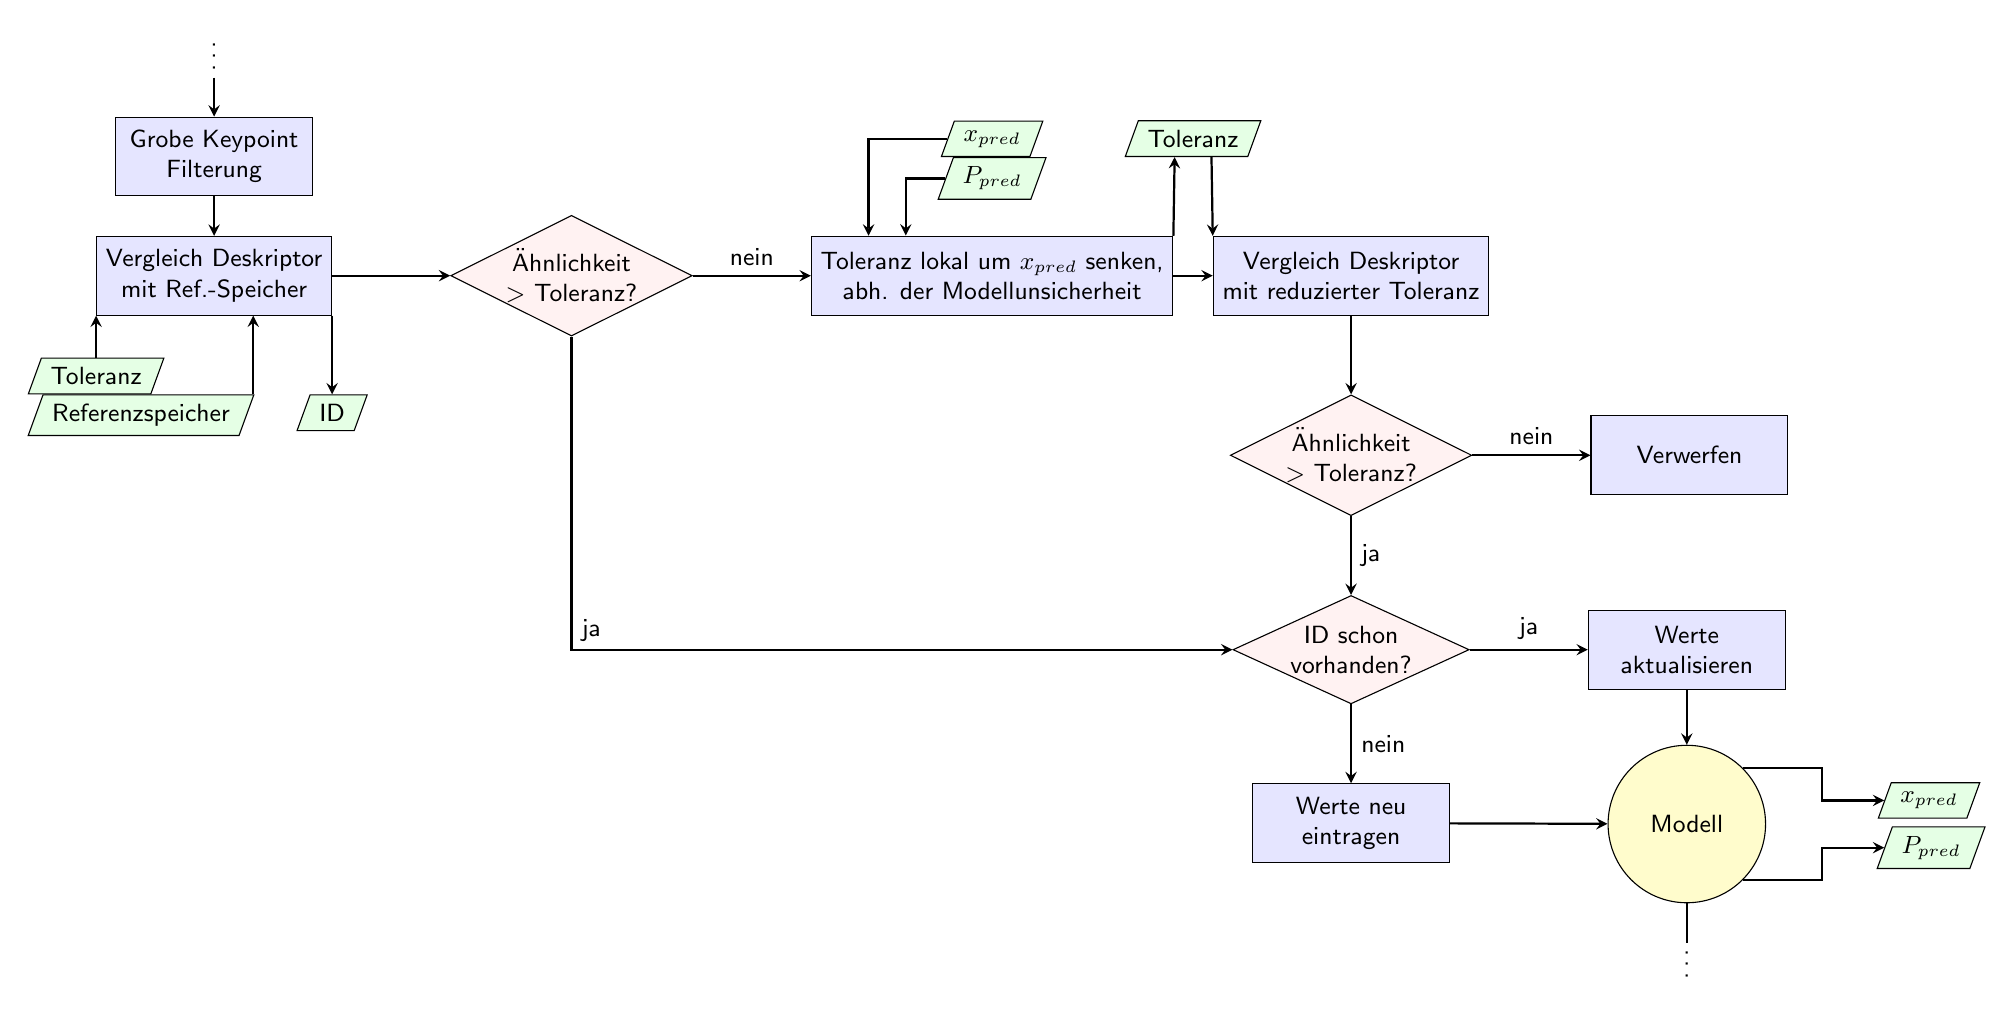
\begin{tikzpicture}[
    node distance=1cm and 1.5cm,
    font=\sffamily\small,
    % Styles für die verschiedenen Formen
    startstop/.style={rectangle, rounded corners, draw, fill=gray!10, minimum width=2cm, minimum height=0.8cm, align=center},
    process/.style={rectangle, draw, fill=blue!10, minimum width=2.5cm, minimum height=1cm, align=center},
    decision/.style={diamond, draw, fill=red!5, aspect=2, inner sep=0pt, minimum width=3cm, align=center},
    data/.style={trapezium, draw, trapezium left angle=70, trapezium right angle=110, fill=green!10, align=center},
    storage/.style={parallelogram, draw, fill=orange!10, minimum width=2cm, align=center},
    % subprocess/.style={circle, draw, fill=yellow!20, minimum size=1.5cm, align=center};
    arrow/.style={thick, ->, >=stealth},
    line/.style={thick, -, >=stealth}
]

% --- Ebene 3: Filterung & Vergleich ---
\node (kp_filter) [process] {Grobe Keypoint\\Filterung};
\node (desc_comp) [process, below=0.5cm of kp_filter] {Vergleich Deskriptor\\mit Ref.-Speicher};
\node (ref_access) [data, below=of desc_comp.south west, xshift=0.57cm] {Referenzspeicher};
\node (tol_access) [data, above=0cm of ref_access, xshift=-0.57cm] {Toleranz};
\node (id_store) [data, below=of desc_comp.south east] {ID};

% --- Ebene 4: Deskriptor Logik ---
\node (desc_tol) [decision, right=of desc_comp] {Ähnlichkeit\\$>$ Toleranz?};

% --- Ebene 4.1: Local Rescue ---
\node (lr) [process, right=of desc_tol] {Toleranz lokal um $x_{pred}$ senken,\\abh. der Modellunsicherheit};
\node (x_access) [data, above=of lr.north] {$x_{pred}$};
\node (P_access) [data, below=0cm of x_access] {$P_{pred}$};
\node (tol_lr_store) [data, above=of lr.north east, xshift=0.25cm] {Toleranz};
\node (desc_comp_lr) [process, right=0.5cm of lr] {Vergleich Deskriptor\\mit reduzierter Toleranz};
\node (desc_tol_2) [decision, below=of desc_comp_lr] {Ähnlichkeit\\$>$ Toleranz?};
\node (discard) [process, right=of desc_tol_2] {Verwerfen};

% --- Ebene 4.2: passt ---
\node (id_exists) [decision, below=of desc_tol_2] {ID schon\\vorhanden?};
\node (update_vals) [process, right=of id_exists] {Werte\\aktualisieren};
\node (entry_vals) [process, below=of id_exists] {Werte neu\\eintragen};

% --- Ebene 5: Modell ---
% \node (Modell) [subprocess, below=of update_vals, yshift=-0.19cm] {Modell};
\node (modell) [circle, draw, fill=yellow!20, minimum size=2cm, below=of update_vals, yshift=0.3cm] {Modell};
\node (x_store) [data, right=of modell, yshift=0.3cm] {$x_{pred}$};
\node (P_store) [data, right=of modell, yshift=-0.3cm] {$P_{pred}$};


% --- Verbindungen ---
\draw [arrow] node[above, anchor=east, rotate=90, xshift=1.65cm] {\dots} ++(0,1) -- (kp_filter.north);

\draw [arrow] (kp_filter) -- (desc_comp);
\draw [arrow] (desc_comp) -- (desc_tol);
\draw [arrow] (tol_access.north) -- (desc_comp.south west);
\draw [arrow] (ref_access.north east) ++(1.16,0) -- ++(0, 1);
\draw [arrow] (desc_comp.south east) -- (id_store.north);

\draw [arrow] (desc_tol) -- node[anchor=south] {nein} (lr);
\draw [arrow] (desc_tol.south) |- node[anchor=west, yshift=0.25cm] {ja} (id_exists);

\draw [arrow] (x_access.west) -- ++(-1,0) -- ++(0, -1.23);
\draw [arrow] (P_access.west) -- ++(-0.5,0) -- ++(0, -0.725);
\draw [arrow] (lr.north east) -- (tol_lr_store.south west);
\draw [arrow] (lr) -- (desc_comp_lr);
\draw [arrow] (tol_lr_store.south east) -- (desc_comp_lr.north west);
\draw [arrow] (desc_comp_lr) -- (desc_tol_2);
\draw [arrow] (desc_tol_2) -- node[anchor=south] {nein} (discard);
\draw [arrow] (desc_tol_2) -- node[anchor=west] {ja} (id_exists);

\draw [arrow] (id_exists) -- node[anchor=south] {ja} (update_vals);
\draw [arrow] (id_exists) -- node[anchor=west] {nein} (entry_vals);

\draw [arrow] (entry_vals) -- (modell);
\draw [arrow] (update_vals) -- (modell);

\draw [arrow] (modell.north east) -- ++(1,0) |- (x_store.west);
\draw [arrow] (modell.south east) -- ++(1,0) |- (P_store.west);

\draw [line] (modell.south) -- ++(0,-0.5) node[below, anchor=east, rotate=90, xshift=0.1cm] {\dots};

\end{tikzpicture}
\end{document}